\documentclass{beamer}
\usetheme{metropolis}
% \usepackage{lmodern}
% \usepackage[margin=1in]{geometry}
% \usepackage{amsmath,amsthm,amssymb,amsfonts, fancyhdr, color, comment, cancel, graphicx, environ}
\usepackage{fontspec}
\setsansfont{Latin Modern Sans}
\usepackage{amsfonts, amsmath, amssymb, amsthm} % AMS Math Packages
\usepackage{mathtools} % Mathematical tools for amsmath
\usepackage{color} % Color control
\usepackage{colortbl} % Color to tables
\usepackage{graphicx} % Enhanced support for graphics 
% \usepackage{algorithm, algpseudocode}
\usepackage[linesnumbered, lined, boxed, commentsnumbered]{algorithm2e} % Algorithms creation
\usepackage{parskip, setspace} % Paragraph indentation and line spacing
\usepackage{xcolor, soul}
\usepackage{mdframed}
\usepackage{array}
% \usepackage[shortlabels]{enumitem}
\usepackage{indentfirst}
\usepackage{hyperref}
\usepackage{tikz}
\usetikzlibrary{shapes.geometric}
\usepackage{listings}
\usepackage{booktabs}
\usepackage{adjustbox}

\definecolor{customgray}{rgb}{0.90, 0.90, 0.90}
\lstdefinestyle{mystyle}{
    backgroundcolor=\color{customgray},
    basicstyle=\ttfamily\footnotesize,
    breakatwhitespace=false,
    breaklines=true,
    captionpos=b,
    keepspaces=true,
    showspaces=false,
    showstringspaces=false,
    showtabs=false
    tabsize=2
}

\setlength\parindent{0pt}
\DeclarePairedDelimiter\ceiling{\lceil}{\rceil}
\DeclarePairedDelimiter\floor{\lfloor}{\rfloor}

\renewcommand{\baselinestretch}{1.25}
\lstset{style=mystyle}

\title{Section 2 Supplement}
\subtitle{CPSC 365: Algorithms}
\author{Amy Zhao}
\date{February 3, 2024}

\definecolor{DocBlue}{RGB}{40, 64, 139}
\setbeamercolor{frametitle}{bg=DocBlue}

\begin{document}
\sethlcolor{teal}
\begin{frame}
    \titlepage
\end{frame}

\begin{frame}
    \frametitle{Outline}
    \footnotesize
    \tableofcontents[sections={1}]
\end{frame}

\section{Divide and Conquer}
\subsection{Main Idea}
\begin{frame}
    \frametitle{Divide and Conquer: Main Idea}
    \begin{enumerate}
        \item Divide the input into smaller subproblems. 
        \item Conquer the subproblems recursively. 
        \item Combine the solutions for the subproblems into a solution for the original problem. 
    \end{enumerate}
    All divide and conquer algorithms follow a similar format: start with the entire input data and make a comparison of two values. Depending on this comparison, determine which portion of the input data to recurse on. 
\end{frame}

\subsection{Partitioning, Medians, Quicksort, and Quickselect}
\begin{frame}
    \frametitle{Divide and Conquer: Quicksort}
    \textbf{Main Idea:} Divide the array on a pivot element which is positioned in a way such that elements less than the pivot are kept on the left side, and elements greater than the pivot are kept on the right side. \\[1em]
    Recurse on each side until the subarrays become single elements before combining. \\[1em]
    \textbf{Time Complexity:} $O(n^2)$ (worst case); $O(n\log n)$ (average case)
\end{frame}

\begin{frame}
\IncMargin{2em}
\begin{algorithm}[H]
    \scriptsize
    \setstretch{1.125}
    \DontPrintSemicolon
    \SetKwData{Left}{left}\SetKwData{This}{this}\SetKwData{Up}{up}
    \SetKwProg{Fn}{Function}{:}{}
    \SetKwFunction{Quicksort}{Quicksort}
    \SetKwFunction{Partition}{Partition}
    \SetKwInOut{Input}{Input}\SetKwInOut{Output}{Output}
    \BlankLine
    \Fn{\Quicksort{$A$, \upshape leftIndex, \upshape rightIndex}}{
        \uIf{\upshape leftIndex $<$ \upshape rightIndex}{
            pivot $\gets$ \Partition{$A$, \upshape leftIndex, \upshape rightIndex}\;
            \Quicksort{$A$, \upshape leftIndex, \upshape pivot $-$ 1}\; 
            \Quicksort{$A$, \upshape pivot, \upshape rightIndex}\;
        }
    }
    \BlankLine \BlankLine
    \Fn{\Partition($A$, \upshape leftIndex, \upshape rightIndex)}{
        set rightIndex as pivot\;
        storeIndex $\gets$ leftIndex $-$ 1
        \BlankLine\BlankLine 
        \For{$i \gets$ \upshape leftIndex $+$ 1 to rightIndex}{
            \uIf{$A[i] < A[\text{\upshape pivot}]$}{
                swap $A[i]$ and $A[\text{storeIndex}]$\; 
                storeIndex $\gets$ storeIndex $+$ 1\;
            }
            swap $A[\text{pivot}]$ and $A[\text{storeIndex} + 1]$\; 
        }
        \Return{\upshape storeIndex $+$ 1}
    }
\end{algorithm}\DecMargin{2em} 
\end{frame}

\begin{frame}
    \frametitle{Divide and Conquer: Quickselect}
    \textbf{Main Idea:} Quickselect uses the same overall approach as quicksort to find the $k$th smallest element in an unordered list. \\[1em]
    It chooses a pivot element and partitions the data on the pivot. It only recurses on the side where the target element is.\\[1em]
    \textbf{Time Complexity:} $O(n)$
\end{frame}

\begin{frame}
    \scriptsize
    \begin{enumerate}
        \item Divide the $n$ elements of $A$ into $\lfloor \frac{n}{5}\rfloor$ groups of five elements each. Add the additional elements to their own group of size $n \text{ mod } 5$. 
        \item Find the median of each group. 
        \item Use the algorithm recursively to find the median (denote it with $x$) of the medians found in the previous step. 
        \item Partition $A$ around $x$ (reorder the elements of $A$ in place so that all elements prior to $x$ are less than $x$). Let $k = \text{rank}(x)$.
        \begin{center}
            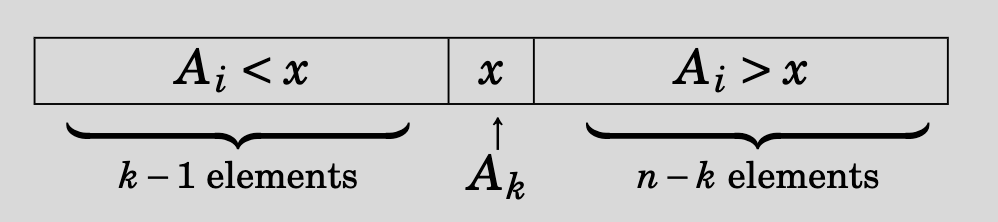
\includegraphics[scale=0.3]{qs_diagram.png}
        \end{center}
        \item Recursively call the algorithm on the appropriate part of the array. 
        \begin{itemize}
            \scriptsize
            \item If $i = k$, return $x$. 
            \item If $i < k$, recursively call the algorithm on $A[1, \dots k-1]$ with target order $i$.
            \item If $i > k$, recursively call the algorithm on $A[k + 1, \dots i]$ with new target order $i - k$. 
        \end{itemize}
    \end{enumerate}
\end{frame}

\begin{frame}{Quickselect: Time Complexity}
    The non-recursive steps all take $O(n)$ time. \\[1em]
    Notice that the recursive call to find the median of medians takes input data of size $\lceil \frac{n}{5} \rceil$ elements. How do we analyze the runtime for the recursive call in step 5? \\[1em]
    WLOG, assume that we need to recurse on the elements larger than the median of medians $x$. 
\end{frame}
\begin{frame}
   \begin{center}
        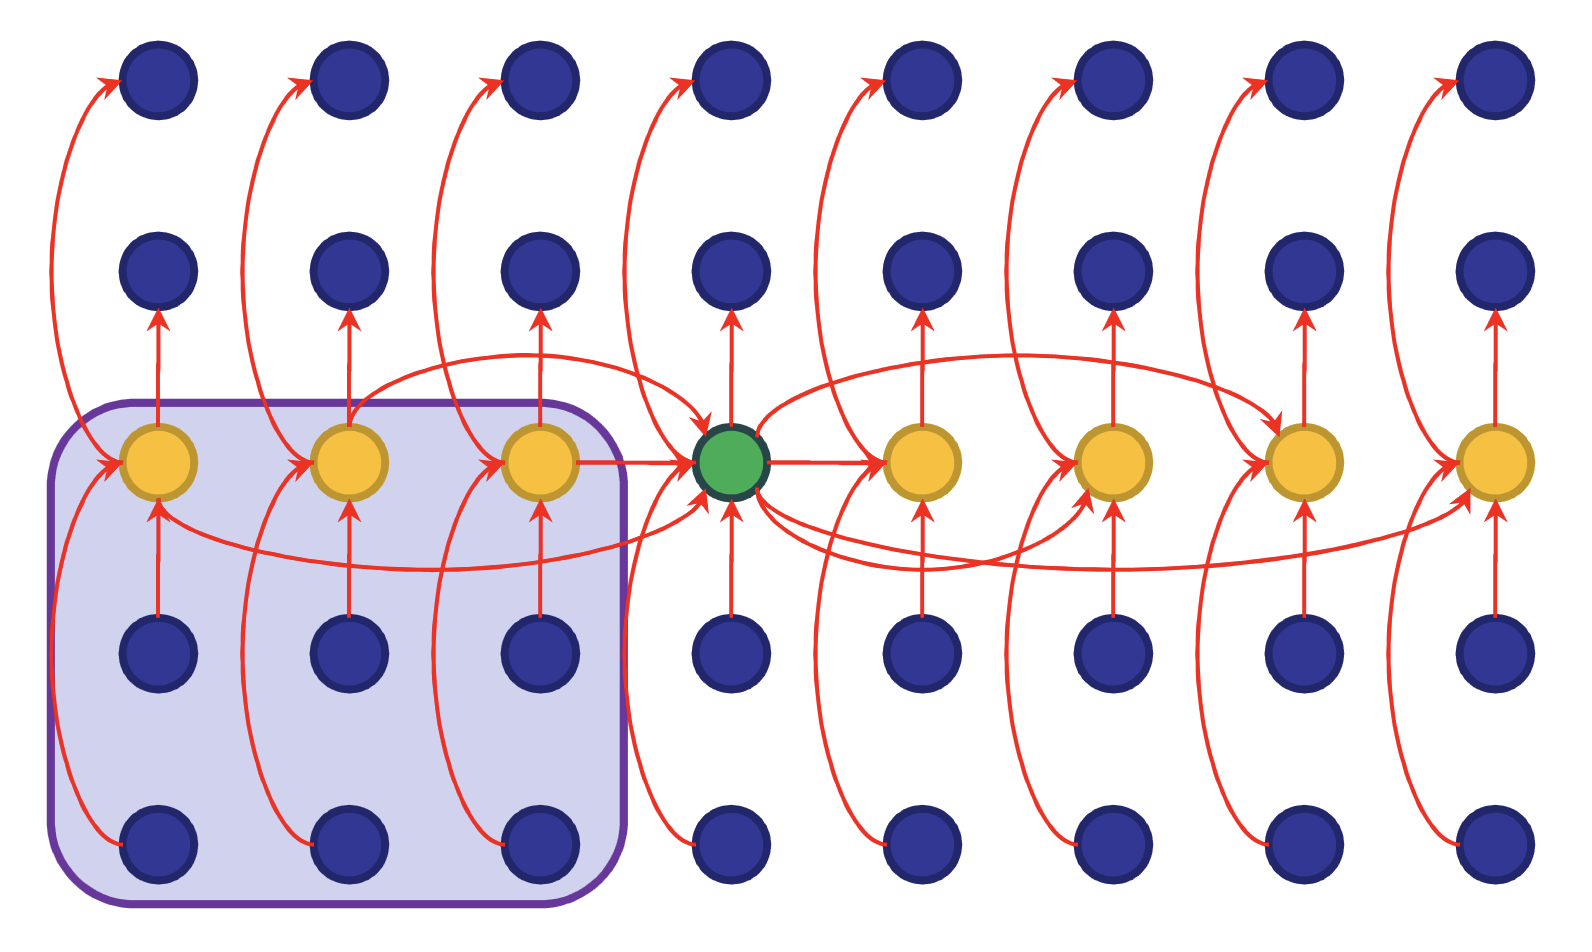
\includegraphics[scale=0.17]{select_example.png}
   \end{center}
   In the diagram, the median of each group is shown in yellow, and $x$ is shown in green. The smaller elements point to the larger elements. \\[1em]
   In general, there are $\lceil \frac{n}{5} \rceil$ groups, which implies there are $\lfloor \frac{1}{2} \lceil \frac{n}{5} \rceil \rfloor$ groups with median at most $x$, and $\lfloor \frac{1}{2} \lceil \frac{n}{5} \rceil \rfloor - 1$ groups with median less than $x$. 
\end{frame}
\begin{frame}
    Each group contributes three elements less than $x$, so we have 
    \begin{align*}
        3 \left( 
            \left\lfloor\dfrac{1}{2}  \left\lceil \dfrac{n}{5} \right\rceil  \right\rfloor - 1 \right) &\geq 3 \left( 
                \left\lfloor\dfrac{n}{10}\right\rfloor - 1 \right) \\
                &= 3 \left(\frac{n}{10} - 2\right) = \frac{3n}{10} - 6
    \end{align*}
    minimum total number of elements less than $x$, and $\frac{7n}{10} + 6$ elements greater than $x$. Therefore, our recurrence is: 
    \begin{gather*}
        T(n) = O(n) + T \left(\frac{n}{5}\right) + T \left(\frac{7n}{10}\right)
    \end{gather*}
\end{frame}
\begin{frame}
    We can solve this recurrence through substitution. Assume $T(n) < cn$:
    \begin{gather*}
        T(n) = an + T\left(\frac{n}{5}\right) + T\left(\frac{7n}{10}\right) \\
        cn \geq c \left(\frac{n}{5}\right) + c\left(\frac{7n}{10}\right) + an \\
        c \geq \frac{9c}{10} + a \Longrightarrow \frac{c}{10} \geq a  \Longrightarrow c \geq 10 a 
    \end{gather*}
    Thus, $T(n) = O(n)$. 
\end{frame}

% % TODO: Proof and the 3/10 7/10 diagram.

\subsection{Mergesort}
\begin{frame}
    \frametitle{Divide and Conquer: Mergesort}
    \textbf{Main Idea:} Divide the array into smaller subarrays, sort each subarray, and merge the sorted subarrays back together. \\[1em]
    At each iteration, the algorithm contains two recursive calls because both subarrays need to be sorted. \\[1em]
    \textbf{Time Complexity:} $O(n\log n)$
\end{frame}

\begin{frame}
\begin{center}
    \resizebox*{!}{0.95\textheight}{
        \IncMargin{2em}
        \begin{algorithm}[H]
            \scriptsize
            \setstretch{1.125}
            \DontPrintSemicolon
            \SetKwProg{Fn}{Function}{:}{}
            \SetKwFunction{Mergesort}{Mergesort}
            \SetKwInOut{Input}{Input}\SetKwInOut{Output}{Output}
            \BlankLine
            \Fn{\Mergesort{$A$, $n$}}{
                \uIf{$n > 1$}{
                    $r \gets \frac{n}{2}$ \; 
                    $L \gets A[:r]$, $M \gets A[r:]$\; 
                    \BlankLine \BlankLine 
                    \Mergesort{$L$, $r$} \; 
                    \Mergesort{$M$, $r$} \;
                    \BlankLine \BlankLine 
                    $i \gets 0$, $j \gets 0$, $k \gets 0$\; 
                    \BlankLine \BlankLine
                    \While{$i < r$ and $j < r$}{
                        \uIf{$L[i] < M[j]$}{
                            $A[k] \gets L[i]$, $i \gets i + 1$\;
                        }
                        \uElse{$A[k] \gets M[j]$, $j \gets j + 1$\;}
                        $k \gets k + 1$ \;
                    }
                    \BlankLine \BlankLine 
                    \While{$i < r$}{
                        $A[k] \gets L[i]$, $i \gets i + 1$, $k \gets k + 1$\;
                    }
                    \BlankLine\BlankLine
                    \While{$j < r$}{
                        $A[k] \gets M[j]$, $j \gets j + 1$, $k \gets k + 1$ 
                    }
                }
            }
        \end{algorithm}\DecMargin{2em} 
    }
\end{center}
\end{frame}

\subsection{Counting Inversions}
\begin{frame}
    \frametitle{Divide and Conquer: Counting Inversions}
    \textbf{Main Idea:} Divide the array into two subarrays, and recursively count the inversions in each half. In the step to combine, count inversions where $a_i$ and $a_j$ are in different halves, and return the sum of the three quantities. \\[1em]
    \textbf{Time Complexity:} $O(n \log n)$
\end{frame}

\begin{frame}
    Suppose we divide array $A$ into $L$ and $R$ subarrays. There are three cases for an inversion $(i, j)$: 
    \begin{itemize}
        \item $i \in L$ and $j \in R$ 
        \item $i \in L$ and $j \in L$ 
        \item $i \in R$ and $j \in R$
    \end{itemize}
    We need to handle case one differently. 
\end{frame}

\begin{frame}
    \begin{center}
        \resizebox*{!}{0.95\textheight}{
            \IncMargin{2em}
            \begin{algorithm}[H]
                \footnotesize
                \setstretch{1.125}
                \DontPrintSemicolon
                \SetKwProg{Fn}{Function}{:}{}
                \SetKwFunction{len}{len}
                \SetKwFunction{CaseOne}{CaseOne}
                \SetKwFunction{CountInversions}{CountInversions}
                \SetKwInOut{Input}{Input}\SetKwInOut{Output}{Output}
                \BlankLine
                \Fn{\CaseOne{$L$, $R$}}{
                   answer $\gets$ 0, $j \gets 0$\; 
                   \BlankLine \BlankLine
                   \For{$i$ \upshape in 0 to \len{$L$} $-$ 1}{
                        \While{$j < $ \len{$R$} \upshape and $R[j] < L[i]$}{
                            $j \gets j + 1$\; 
                        }
                        $\text{answer} \gets \text{answer} + j$\; 
                   }
                   \BlankLine \BlankLine 
                   \Return{\upshape answer}
                }
                \BlankLine \BlankLine 
                \Fn{\CountInversions{$A$, $n$}}{
                    \uIf{$n \leq 1$}{\Return{0}\;}
                    \BlankLine 
                    $L \gets A\left[: \frac{n}{2} - 1\right]$, $R \gets A\left[\frac{n}{2}:\right]$\; 
                    \BlankLine 
                    answer $\gets$ \CountInversions{$L$, \len{$L$}} \;
                    answer $\gets$ answer $+$ \CountInversions{$R$, \len{$R$}}\;
                    answer $\gets$ answer $+$ \CaseOne{$L$, $R$}\;
                    \BlankLine \BlankLine
                    \Return{\upshape answer}
                }
               
            \end{algorithm}\DecMargin{2em} 
        }
    \end{center}
\end{frame}

\subsection{Closest Pair of Points}
\begin{frame}
    \frametitle{Divide and Conquer: Closest Pair}
    \textbf{Main Idea:} Compute a vertical line that roughly divides the points in half. Find the closest pair in each side recursively, and find the closest pair with one point in each side. Return the best of three solutions. \\[1em]
    \textbf{Time Complexity:} $O(n \log^2(n))$, but can be reduced to $O(n \log n)$
\end{frame}

% TODO: Code for closes pair of points
\begin{frame}
    \begin{center}
        \resizebox*{!}{0.95\textheight}{
            \IncMargin{2em}
            \begin{algorithm}[H]
                \scriptsize
                \setstretch{1.125}
                \DontPrintSemicolon
                \SetKwProg{Fn}{Function}{:}{}
                \SetKwFunction{ClosestPair}{ClosestPair}
                \SetKwFunction{ClosestPairRec}{ClosestPairRec}
                \SetKwFunction{dist}{dist}
                \SetKwInOut{Input}{Input}\SetKwInOut{Output}{Output}
                \BlankLine
                \Fn{\ClosestPair{$P$}}{
                    $P_x \gets$ $P$ sorted by $x$-coordinate \;
                    $P_y \gets$ $P$ sorted by $y$-coordinate \;
                    $(p_0^*, p_1^*) \gets$ \ClosestPairRec{$P_x$, $P_y$}\;
                }
                \BlankLine\BlankLine 
                \Fn{\ClosestPairRec{$P_x$, $P_y$}}{
                    \uIf{$|P| \leq 3$}{\Return{closest pair through computation}}
                    \BlankLine \BlankLine 

                    $Q \gets$ first $\ceiling*{\frac{n}{2}}$ points in $P_x $, $Q_x \gets$ $Q$ sorted by $x$-coordinate, $Q_y \gets$ $Q$ sorted by $y$-coordinate \; 
                    \BlankLine
                    $R \gets$ remaining $\floor*{\frac{n}{2}}$ points in $P_x$, $R_x \gets$ $R$ sorted by $x$-coordinate, $R_y \gets$ $R$ sorted by $y$-coordinate \;

                    \BlankLine \BlankLine 
                    $(q_0^*, q_1^*) \gets$ \ClosestPairRec{$Q_x$, $Q_y$} \; 
                    $(r_0^*, r_1^*) \gets$ \ClosestPairRec($R_x$, $R_y$) \;
                    
                    \BlankLine \BlankLine 
                    $\delta \gets \min\{\dist{$q_0^*, q_1^*$}, \dist{$r_0^*, r_1^*$}\}$ \; 
                    $x^* \gets$ maximum $x$-coordinate $\in Q$\; 

                    \BlankLine \BlankLine 
                    $L \gets \{(x, y): x = x^*\}$ \; 
                    $S \gets$ points $\in P$ within distance $\delta$ of $L$, $S_y \gets$ $S$ sorted by $y$-coordinate\; 

                    \BlankLine \BlankLine 
                    \For{$s \in S_y$}{
                        compute distance from $s$ to next 15 points in $S_y$\; 
                        $(s, s') \gets$ pair which achieves minimum distance\;  
                    }
                    \BlankLine \BlankLine
                    \uIf{$\dist{$s, s'$} < \delta$}{\Return{$(s, s')$}}
                    \uElseIf{$\dist{$q_0^*, q_1^*$} < \dist{$r_0^*, r_1^*$}$}{\Return{$(q_0^*, q_1^*)$}}
                    \uElse{\Return{$(r_0^*, r_1^*)$}}
                }
            \end{algorithm}\DecMargin{2em} 
        }
    \end{center}
\end{frame}

% \begin{frame}
%     \begin{center}
%         \resizebox*{!}{0.95\textheight}{
%             \IncMargin{2em}
%             \begin{algorithm}[H]
%                 \footnotesize
%                 \setstretch{1.125}
%                 \DontPrintSemicolon
%                 \SetKwProg{Fn}{Function}{:}{}
%                 \SetKwFunction{ClosestPair}{ClosestPair}
%                 \SetKwInOut{Input}{Input}\SetKwInOut{Output}{Output}
%                 \BlankLine
%                 \Fn{\ClosestPair{$p_1, \dots, p_n$}}{
%                     compute line $L$ such that $\frac{n}{2}$ points are on each side\; 
%                     $\delta_1 \gets$ \ClosestPair{left half}\; 
%                     $\delta_2 \gets$ \ClosestPair{right half}\;

%                     \BlankLine 
%                     delete all points further than $\delta$ from $L$\; 
%                     sort remaining points \; 

%                     \BlankLine
%                     scan through points and compare distance \; 

%                     \uIf{$\text{\upshape distance} < \delta$}{$\delta \gets \text{distance}$}
%                     \BlankLine
%                     \Return{\delta}

%                 }
               
%             \end{algorithm}\DecMargin{2em} 
%         }
%     \end{center}
% \end{frame}

\subsection{Strassen's Algorithm}
\begin{frame}
    \frametitle{Divide and Conquer: Strassen's Algorithm}
    \textbf{Main Idea:} Divide the two matrices into smaller sub-matrices, and calculate the values recursively.
    \footnotesize
    \begin{gather*}
        \begin{pmatrix}
            A & B \\ C & D
        \end{pmatrix}
        \begin{pmatrix}
            E & F \\ G & H
        \end{pmatrix} = \begin{pmatrix}
            S_1 + S_2 - S_4 + S_6 & S_4 - S_5 \\
            S_6 + S_7 & S_2 - S_3 + S_5 - S_7
        \end{pmatrix}
    \end{gather*}
    \begin{center}
        \begin{tabular}{lll}
            $S_1 = (B-D)(G+H)$ & $S_2 = (A+D)(E+H)$ & $S_3 = (A-C)(E+F)$ \\
            $S_4 = (A+B)H$ & $S_5 = A(F-H)$ & $S_6 = D(G-E)$ \\
            $S_7 = (C+D)E$ \\
        \end{tabular}
    \end{center}
    \normalsize
    \textbf{Time Complexity:} $O(n^{\log_2 7})$ 
\end{frame}

\begin{frame}
\begin{center}
    \resizebox*{0.95\textwidth}{!}{
        \IncMargin{2em}
        \begin{algorithm}[H]
            \scriptsize
            \setstretch{1.125}
            \DontPrintSemicolon
            \SetKwProg{Fn}{Function}{:}{}
            \SetKwFunction{Strassen}{Strassen}
            \SetKwInOut{Input}{Input}\SetKwInOut{Output}{Output}
            \BlankLine
            \Fn{\Strassen{$M$, $N$}}{
                \uIf{$M$ \upshape $1 \times 1$}{
                    \Return{$M_{11}N_{11}$}
                }
    
                \BlankLine \BlankLine 
                $M \gets \begin{pmatrix}
                    A & B \\ C & D
                \end{pmatrix}$, $N \gets \begin{pmatrix}
                    E & F \\ G & H
                \end{pmatrix}$ \;
    
                \BlankLine \BlankLine
                $S_1 \gets$ \Strassen{$B - D$, $G + H$}\;
                $S_2 \gets$ \Strassen{$A + D$, $E + H$}\; 
                $S_3 \gets$ \Strassen{$A - C$, $E + F$}\;
                $S_4 \gets$ \Strassen{$A + B$, $H$}\; 
                $S_5 \gets$ \Strassen{$A$, $F - H$}\; 
                $S_6 \gets$ \Strassen{$D$, $G - E$}\; 
                $S_7 \gets$ \Strassen{$C + D$, $E$}\;
    
                \BlankLine \BlankLine
                \Return{$\begin{pmatrix}
                    S_1 + S_2 - S_4 + S_6 & S_4 - S_5 \\ S_6 + S_7 & S_2 - S_3 + S_5 - S_7
                \end{pmatrix}$}
            }
            
        \end{algorithm}\DecMargin{2em} 
    }
\end{center}
\end{frame}

\subsection{Karatsuba's Algorithm}
\begin{frame}
    \frametitle{Divide and Conquer: Karatsuba's Algorithm}
    \footnotesize
    \textbf{Main Idea:} Given two integers (in base-2), perform three recursive multiplications. It relies on the fact that the two integers can be written as lower order and higher order bits:
    \begin{gather*}
        x = x_1 \cdot 2^{\frac{n}{2}} + x_0 \\
        y = y_1 \cdot 2^\frac{n}{2} + y_0 
    \end{gather*}
    The product becomes the following: 
    \begin{align*}
        xy &= (x_1 \cdot 2^{\frac{n}{2}} + x_0) ( y_1 \cdot 2^\frac{n}{2} + y_0) \\
        &= x_1y_1 \cdot 2^n + (x_1 y_0 + x_0 y_1) \cdot 2^{\frac{n}{2}} + x_0 y_0
    \end{align*}
    \textbf{Time Complexity:} $O(n^{\log_2 3})$
\end{frame}

\begin{frame}
    \IncMargin{2em}
    \begin{algorithm}[H]
        \footnotesize
        \setstretch{1.125}
        \DontPrintSemicolon
        \SetKwProg{Fn}{Function}{:}{}
        \SetKwFunction{FasterMultiplication}{FasterMultiplication}
        \SetKwInOut{Input}{Input}\SetKwInOut{Output}{Output}
        \BlankLine
        \Fn{\FasterMultiplication{$x$, $y$}}{
            write $x$ as $x_1 \cdot 2^{\frac{n}{2}} + x_0$\; 
            write $y$ as $y_1 \cdot 2^{\frac{n}{2}} + y_0$\; 

            \BlankLine \BlankLine
            $x_{10} \gets x_1 + x_0$ \; 
            $y_{10} \gets y_1 + y_0$ \;
            
            \BlankLine \BlankLine
            $p \gets$ \FasterMultiplication{$x_{10}$, $y_{10}$}\; 
            $x_1y_1 \gets$ \FasterMultiplication{$x_1$, $y_1$}\; 
            $x_0y_0 \gets$ \FasterMultiplication{$x_0$, $y_0$}\; 
            
            \BlankLine \BlankLine
            \Return{$x_1y_1 \cdot 2^n + (p-x_1y_1 - x_0y_0) \cdot \frac{n}{2} + x_0y_0$}
        }
    \end{algorithm}\DecMargin{2em} 
\end{frame}

\end{document}